%%%%% Kompendium -- Wellen und Optik %%%%%
%% Wellen -- Eigenschaften und Phänomene %%


%Some sample text to be displayed above the first subsection

%\subsection{Prinzip}

%Ein Zyklotron besteht aus Zwei hohlen, halbzylindrischen und Duanden an denen eine Spannung mit unterschiedlichem Vorzeichen anliegt, und darüber bzw. darunter liegende Magneten, die ein homogenes Magnetfeld erzeugen. Zudem gibt es einen Einlass und einen Auslass für Teilchen.

%\begin{wrapfigure}{r}{0.4\textwidth} \label{Zyklo}
%
%	\vspace{-10pt}
%	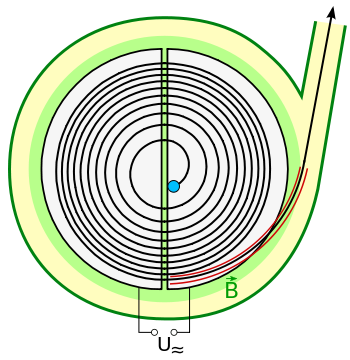
\includegraphics[width=0.35\textwidth]{Zyklotron_Prinzipskizze02.png}
%	\vspace{-13pt}
%	\caption{Prinzipskizze eines Zyklotrons}
%	\vspace{-5pt}	
%	
%\end{wrapfigure}

%\subsubsection{Anwendung}

% Some Formula:

%\begin{equation}
%	x= \frac{y \cdot 13 \pi z}
%			{\cos \alpha}
%\end{equation}

%%%%%%%%%%%%%%%%%%%%%%%
% Eigentlicher Beginn %
%%%%%%%%%%%%%%%%%%%%%%%

Im Folgenden werden bei der Nennung von \glqq Wellen\grqq{} immer Transversalwellen gemeint, wenn es keine weitere Anmerkung gibt.  



\subsection{Reflexion}  

	\paragraph{Fixiertes Ende}
	
	Wenn eine Welle von einem fixierten Ende (eingespannt) reflektiert wird, dann gibt es einen Phasensprung von $180 \degree$ oder $\pi$, bzw $\frac{T}{2}$.
	
	\paragraph{Loses Ende}
	
	Trifft eine Welle auf ein loses Ende, dann wird sie ohne  Phasensprung reflektiert.



\subsection{Überlagerung}

Wenn sich Wellen in einem räumlichen Punkt treffen, dann überlagern sie sich und bilden eine summierte Welle. Wenn also ein Wellenberg auf einen Wellenberg trifft, addieren sich beide Welle und der resultierende Wellenberg ist höher. Sollte auf einen Wellenberg ein Wellental treffen wird auf addiert, und die resultierende Welle von der Amplitude her kleiner.

Nachdem sich die Wellen in diesem Punkt überlagert haben, laufen beide weiter ohne die andere zu beeinflussen; so als hätte es die Überlagerung nie gegeben.

	\subsubsection{Stehende Welle}
	
	Wenn sich gegenläufige, das heißt parallel und identisch, aber in die entgegengesetzte Richtung fortschreitende, Wellen mit derselben Wellenlänge überlagern, entsteht eine stehende Welle. 
	Das heißt, dass es mindestens 2 Oszillatoren auf dieser Welle gibt, die sich gar nicht bewegen (\glqq stehen\grqq), die sogenannten Knotenpunkte.
	
	Eine stehende Welle kann zum Beispiel ausgelöst werden, wenn bei einer Reflexion am festen Ende die Hälfte der Wellenlänge $\lambda$ ein ganzzahliges Vielfaches der Abstands $l$ der beiden Enden ist. $k$ ist in diesem Fall eine Variable, die nur positive ganze Zahlen annehmen kann:
	
	\begin{equation} \label{stehendewelle}
		\lambda = 2k \cdot l \ \ \ wobei \ \ k \in 1,2,3...
	\end{equation}



\subsection{Interferenzen} \label{sec:interferenz}

Wenn sich Wellen, die nicht nur dieselbe Wellenlänge, sondern auch die selbe Amplitude aufweisen, in einem Punkt überlagern, dann kann es zu Interferenzen kommen.

	\subsubsection{Konstruktive Interferenz}
	
	Wenn in dem Punkt beide Wellen ein Maximum aufweisen, sich also zu einem höheren Wellenberg addieren, spricht man von konstruktiver Interferenz.
	
	Dazu muss der Gangunterschied $\delta$ ein ganzzahliges Vielfaches der Wellenlänge sein:
	
	\begin{equation}	\label{eq:kon_interferenz}
		\delta = k \cdot \lambda \ \ \ wobei \ \ k \in 1,2,3...
	\end{equation}
	
	\subsubsection{Destruktive Interferenz}
	
	Im Gegensatz zur konstruktiven Interferenz, treffen nun also Wellen aufeinander, die einmal einen Wellenberg und einmal ein Wellental aufweisen. Da sie dieselbe Amplitude haben, ist die resultierende Amplitude im betroffenen Punkt $0$.
	
	Der Gangunterschied $\delta$ muss daher die Summe eines ganzzahliges Vielfaches Wellenlänge und der halben Wellenlänge sein:
	
	\begin{equation}
		\delta = k \cdot \lambda + \frac{\lambda}{2} \ \ \ wobei \ \ k \in 1,2,3...
	\end{equation}

	Zur einfacheren Umstellung nach $\lambda$ existiert diese, internationale Form:
	
	\begin{equation} \label{eq:des_interferenz}
		\delta = (2k -1) \cdot \frac{\lambda}{2} \ \ \ wobei \ \ k \in 1,2,3...
	\end{equation}



\subsection[Ausbreitung in Elementarwellen]{Ausbreitung in Elementarwellen (Huygens'sches Prinzip)} \label{subsec:ausbreitung}

Das Huygens'sche Prinzip macht eine wichtige Aussage zur Ausbreitung von Wellen:

\glqq Jedes Teilchen (Oszillator), das von einer Wellenfront erfasst wird, löst von sich aus eine zirkulare Welle nach allen Seiten aus.\grqq{} Die eigentlich sichtbare Wellenfront ist nach Huygens eine Einhüllende aller \glqq Elementarwellen\grqq . Dadurch ist es Wellen unter anderem möglich in den geometrischen Schattenraum zu propagieren. \referenz{subsec:doppelspalt}


\subsection{Wellen am Doppelspalt} \label{subsec:doppelspalt}

Wenn nun eine räumlich und zeitlich kohärente Wellen, das heißt Wellenfronten deren Wellen sowohl parallel als auch phasengleich (mit derselben Wellenlänge und Gangunterschied $\delta= k \cdot \lambda$) verlaufen, auf ein Hindernis mit 2 schmalen Spalten trifft, bildet sich folgendes Interferenzmuster:

%\begin{figure}[h!]
%	\center
%	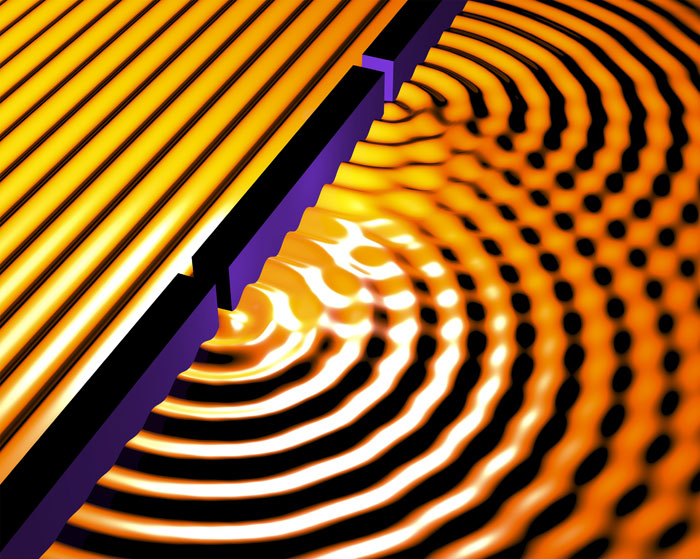
\includegraphics[width=0.4\textwidth]{doppelspalt_wasser}
%	\caption{Eine kohärente Welle am Doppelspalt}
%\end{figure}

Dies ist mit dem Huygens'schen Prinzip (\referenz{subsec:ausbreitung}) zu erklären: Angenommen, in jedem Spalt gäbe es nur ein schwingendes Teilchen. Dieses wird von der Wellenfront erfasst und ist selber Auslöser einer zirkularen Wellen. Da dieser Oszillator an dieser Stelle der einzige ist, gibt es keine gerade Wellenfront als Einhüllende, sondern einzig die Zirkularwelle des angeregten Oszillators.


\subsubsection{Mathematisierung}

	Der Versuch ist auch mit Laserlicht, also Monochromatisch (eine einzige Wellenlänge) und Kohärent, durchführbar. Das Licht wird durch einen schmalen Doppelspalt mit dem Spaltabstand $d \leq 2mm$ hinter dem sich im Abstand $a$ ein Schirm befindet. 
	
	Auf dem Schirm ist ein Interferenzmuster zu beobachten. In der Mitte ist ein heller Streifen, links und rechts davon, symmetrisch, sind weniger intensive Lichtpunkte. Diese Punkte werden Maxima genannt, da in diesen Punkten konstruktive Interferenz herrscht (\referenz{sec:interferenz}). An den Minimalstellen herrschen destruktive Interferenzen. Der Gangunterschied ergibt sich hier durch den Unterschiedlichen Abstand der Punkte auf dem Schirm zu dem beiden Schlitzen.
	
	Eine Zeichnung:
	
%	\begin{figure}[h!]
%		\center
%		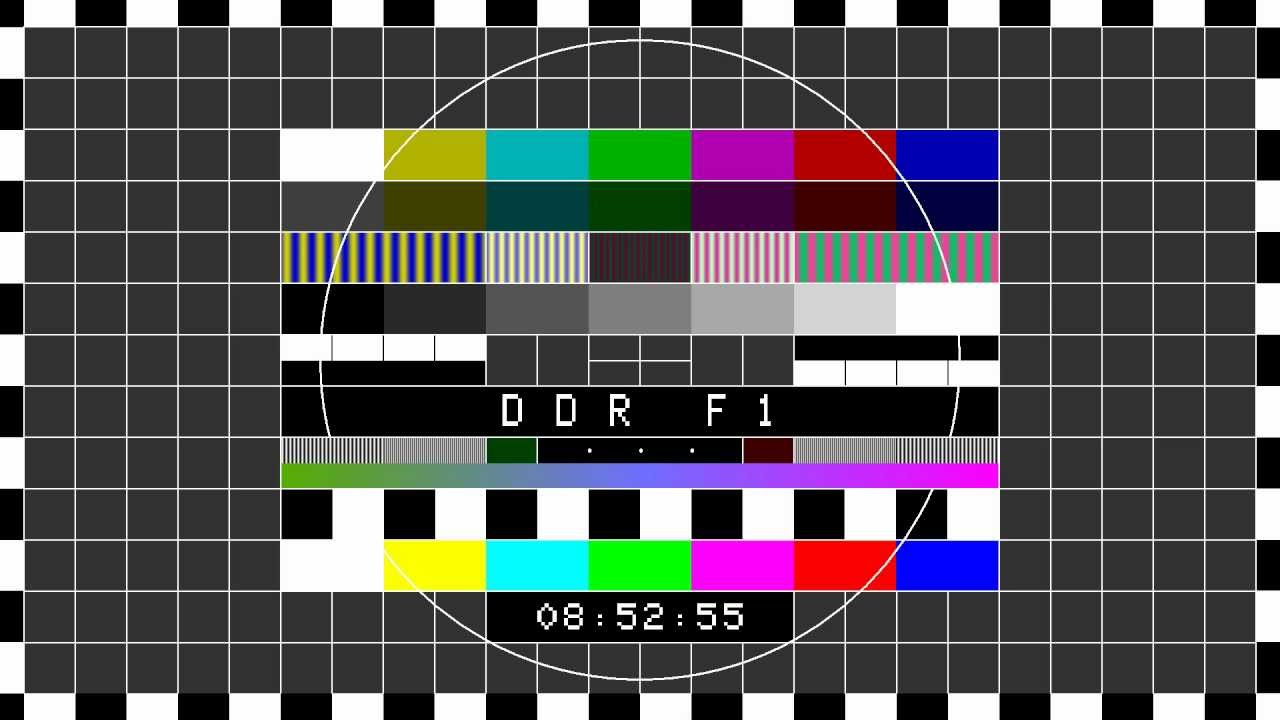
\includegraphics[width=0.8\textwidth]{default}
%		\caption{Das Maxima 1. Ordnung am Doppelspalt}
%	\end{figure}
	
	Die Winkel $\alpha_a$ und $\alpha_d$ sind gleich und werden im Folgen schlicht als $\alpha$ bezeichnet. Für $\alpha$ ergeben sich aus den trigonomischen Winkelfunktionen im rechtwinkligen Dreieck 2 Gleichungen: $sin{\alpha}=\frac{\delta}{d}$ und $tan{\alpha}=\frac{d_k}{a}$. Da $a>>d_k$ ist $\alpha<10 \degree$ und die Kleinwinkelnäherung $sin{\alpha} \approx \tan{alpha}$ kann verwendet werden. Der Gangunterschied $\delta$ muss der Bedingung für konstruktive Interferenz $\delta = k \cdot \lambda$ genügen (Siehe Gleichung \ref{eq:kon_interferenz} auf Seite \pageref{eq:kon_interferenz}). Daraus Ergibt sich:
	
	\begin{align}
		\sin{\alpha} &= \tan{\alpha} \\
		\frac{\delta}{d} &= \frac{d_k}{a} \\
		\frac{k \cdot \lambda}{d} &= \frac{d_k}{a}  \ \ \ wobei \ \ k \in 1,2,3... \\
		\lambda &= \frac{d_{k} \cdot d}{a \cdot k}  \ \ \ wobei \ \ k \in 1,2,3...
	\end{align}
	
	Für $k$ muss die Ordnung des betrachteten Maxima eingesetzt werden.
		

\subsubsection{Ohne Kleinwinkelnäherung}

	Um präziser ablesen zu können, kann ein Gitter statt einem Doppelspalt verwendet werden. Das Gitter weist einen wesentlich geringeren Abstand zwischen den Schlitzen auf (z.B. $\frac{1}{600}mm$), sodass die Interferenzmaxima deutlich weiter auseinander liegen. Der Fakt, dass der Lichtdurchsatz durch das Hinzufügen von mehr Schlitzen zu einem Gitter erhöht wurde, ändert nichts an den mathematischen Grundlagen des Versuchs.
	
	Allerdings geht mit dem größeren Abstand der Punkte auf dem Schirm die Gültigkeit der Kleinwinkelnäherung verloren. Allerdings kann die Größe des Winkels $\alpha_a$ über $\arctan{\frac{d_k}{a}}$ berechnet werden und in die Gleichung $\sin{\alpha} = \frac{\delta}{d}$ eingesetzt werden:
	
	\begin{align}
		\frac{\delta}{d} &= \sin{\alpha} \\
		 \delta &= \sin{(\arctan{\frac{d_k}{a}})} \cdot d \\
		\lambda \cdot k &= \sin{(\arctan{\frac{d_k}{a}})} \cdot d \ \ \ wobei \ \ k \in 1,2,3... \\
		\lambda &= \frac{\sin{(\arctan{\frac{d_k}{a}})} \cdot d}{k} \ \ \ wobei \ \ k \in 1,2,3...
	\end{align}


\subsection{Lichtspektrum am Doppelspalt}

Wenn ein Lichtspektrum (z.B. weißes Licht von einer Glühbirne) auf einen Doppelspalt oder ein Gitter trifft, dann tritt dasselbe Phänomen wie bei monochromatischem Licht, mit dem Unterschied, dass die unterschiedlichen Wellenlängen im Spektrum ihren eigenen, von der Wellenlänge abhängigen, Abstand $d_k$ haben. Dadurch wird das Lichtspektrum von violett bis rot aufgefächert (Dispersion).










